\documentclass[tikz,border=8pt]{standalone}
\usepackage{amsmath}
\usetikzlibrary{arrows.meta}
\definecolor{ink}{HTML}{21352F}
\definecolor{teal}{HTML}{087F7B}
\definecolor{blue}{HTML}{4B77A8}
\definecolor{gold}{HTML}{C58B2A}
\definecolor{rose}{HTML}{B65A62}
\begin{document}
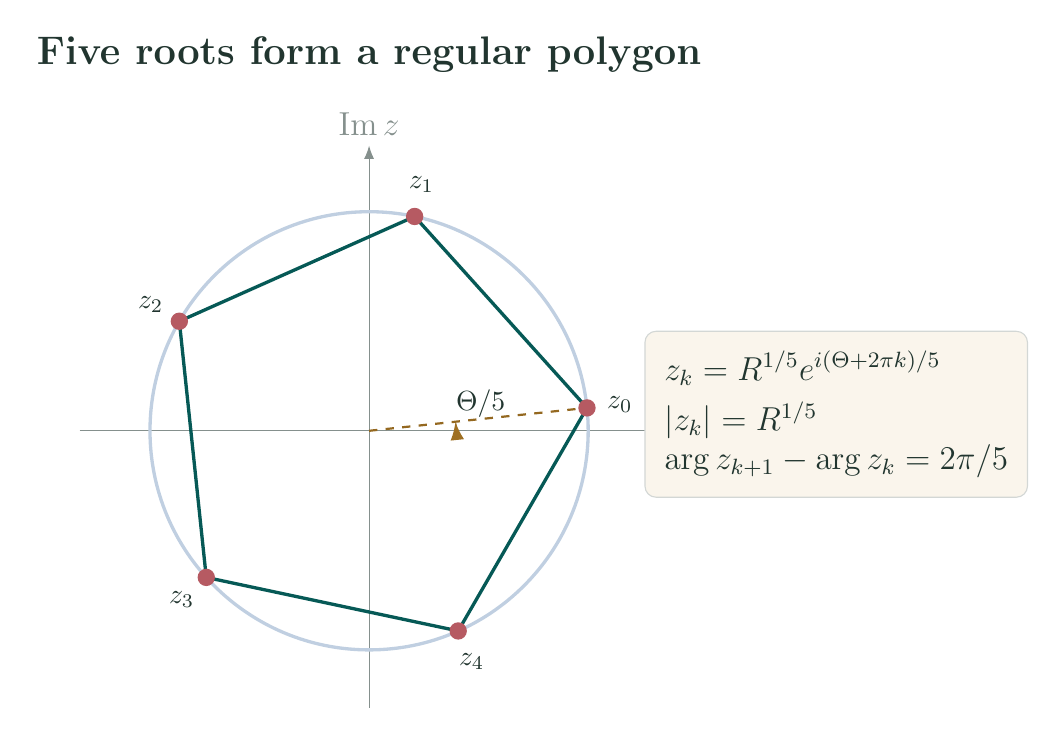
\begin{tikzpicture}[font=\large\sffamily,text=ink,>=Latex,scale=1.05]
  \node[font=\bfseries\Large] at (0,4.55)
    {Five roots form a regular polygon};
  \draw[->,ink!55] (-3.5,0)--(3.65,0) node[right] {$\operatorname{Re}z$};
  \draw[->,ink!55] (0,-3.35)--(0,3.45) node[above] {$\operatorname{Im}z$};
  \draw[blue!35,very thick] (0,0) circle (2.65);
  \draw[gold!75!black,thick,dashed] (0,0)--({2.65*cos(6)},{2.65*sin(6)});
  \draw[teal!70!black,very thick]
    ({2.65*cos(6)},{2.65*sin(6)})
    --({2.65*cos(78)},{2.65*sin(78)})
    --({2.65*cos(150)},{2.65*sin(150)})
    --({2.65*cos(222)},{2.65*sin(222)})
    --({2.65*cos(294)},{2.65*sin(294)})--cycle;
  \foreach \k in {0,...,4}{
    \fill[rose] ({2.65*cos(6+72*\k)},{2.65*sin(6+72*\k)}) circle (.105);
    \node[font=\normalsize,fill=white,inner sep=1.5pt]
      at ({3.05*cos(6+72*\k)},{3.05*sin(6+72*\k)}) {$z_{\k}$};
  }
  \draw[gold!80!black,thick,->] (1.05,0)
    arc[start angle=0,end angle=6,radius=1.05];
  \node[font=\normalsize] at (1.35,.33) {$\Theta/5$};
  \node[draw=ink!20,fill=gold!9,rounded corners=4pt,
        inner sep=7pt,align=left] at (5.65,.2)
    {$\displaystyle z_k=R^{1/5}
       e^{i(\Theta+2\pi k)/5}$\\[4pt]
     $|z_k|=R^{1/5}$\\
     $\arg z_{k+1}-\arg z_k=2\pi/5$};
\end{tikzpicture}
\end{document}
